\documentclass{standalone}
\usepackage{tikz}
\usepackage{tikz-qtree}
\usepackage[makeroom]{cancel}
\usetikzlibrary{fit}


\begin{document} 
	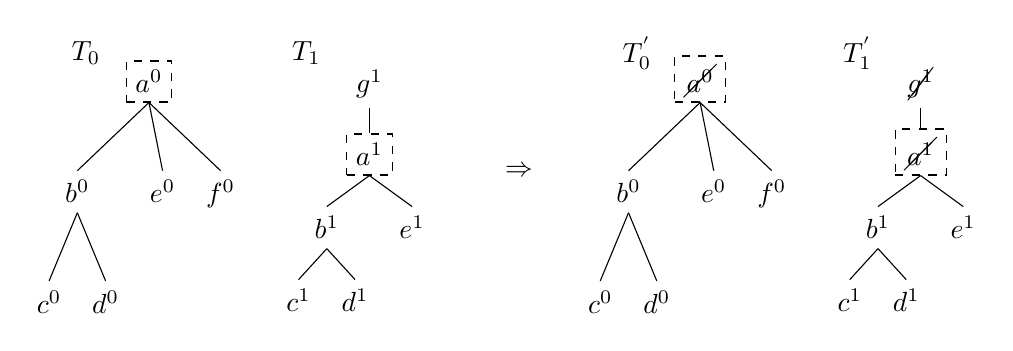
\begin{tikzpicture}[level distance=1.4cm, sibling distance=4.5pt]

	          
		    \node (x) at (-0.8,0.5) {$T_0$};
		    \Tree [.\node[draw,dashed]{$a^0$};
		            [.$b^0$
		                [.$c^0$ ] 
		                [.$d^0$ ] 
		            ] 
		            [.$e^0$ ]
		            [.$f^0$ ]
		          ]

		    

	    \begin{scope}[xshift=2.8cm]
		    \tikzset{level 1+/.style={level distance=2.2\baselineskip}}
			    \node (x) at (-0.8,0.5) {$T_1$} ;
			    \Tree [.$g^1$
				    	  [.\node[draw,dashed]{$a^1$};
				            [.$b^1$
				                [.$c^1$ ] 
				                [.$d^1$ ] 
				            ] 
				            [.$e^1$ ]
				          ]
				      ]
				\node (x) at (1.9,-1) {$\Rightarrow$};
	    \end{scope}


		\begin{scope}[xshift=7.0cm]
		    \node (x) at (-0.8,0.5) {$T_0^{'}$};
		    \Tree [.\node[draw,dashed]{\cancel{$a^0$}};
		            [.$b^0$
		                [.$c^0$ ] 
		                [.$d^0$ ] 
		            ] 
		            [.$e^0$ ]
		            [.$f^0$ ]
		          ]
		\end{scope}

		\begin{scope}[xshift=9.8cm]
		\tikzset{level 1+/.style={level distance=2.2\baselineskip}}
			    \node (x) at (-0.8,0.5) {$T_1^{'}$};
			    \Tree [.\cancel{$g^1$}
				    	  [.\node[draw,dashed]{\cancel{$a^1$}};
				            [.$b^1$
				                [.$c^1$ ] 
				                [.$d^1$ ] 
				            ] 
				            [.$e^1$ ]
				          ]
				      ]
		\end{scope}


	\end{tikzpicture}
\end{document} 